\documentclass[12pt]{article}\pagestyle{myheadings}

\title{DBT Prüfungsfragen}

\markright{DBT Ausarbeitung}
\author{Johannes Spilka}

\usepackage{amsmath,amssymb,amsthm,amsfonts,graphics}
\usepackage{listings}
\usepackage{grffile}
\usepackage{graphicx}
\theoremstyle{plain}
\newtheorem{theorem}{Theorem}
\newtheorem{lemma}[theorem]{Lemma}
\newtheorem{corollary}[theorem]{Corollary}
\newtheorem{proposition}[theorem]{Proposition}
\newtheorem*{definition}{Definition}

\renewcommand{\qedsymbol}{\ensuremath{\blacksquare}}
\newcommand{\N}{\mathbb{N}}
\newcommand{\Z}{\mathbb{Z}}
\newcommand{\Q}{\mathbb{Q}}
\newcommand{\R}{\mathbb{R}}
\newcommand{\C}{\mathbb{C}} 

\begin{document}

\maketitle
\begin{enumerate}

\item \textbf{Discuss the 5 tuning-principals, give examples:} \\
\begin{itemize}
\item think globally, fix logically\\
global denken: das Problem finden und nicht nur dauerweise behandeln\\
lokal fixen mit minimalen Eingriffen um mögliceh sideeffects so gut es geht zu verhindern.\\
Zum Beispiel wenn Festplatte sehr überarbeitet ist was tun ?
\textbf{Lösungsweg a:} Man kauft einfach noch mehr Disks (local thinking)\\
Wenn man global denkt schaut man lieber wo ist die ganze Disk Aktivität generiert?\\
\item[-]fehlt ein index bei einem häufig auftretenden query? (dann fügt man einen query hinzu)
\item[-]der buffer der Datenbank ist zu klein ? so kann man den Buffer erhöhen.
\item[-]Protokoll und häufig genutzte Daten teilen sich die gleiche Festplatte? Einfach das Protokol auf eine andere Disk verschieben.\\
---$>$ Die Ursache zu beheben ist günsiter und effizienter als nur ständig die Symptome zu bekämpfen.\\
\textbf{Lösungsweg b:} Die Query mit der längsten Laufzeit bechleunigen.\\
Die langsamste Query ist vlt die unwichtigste und bringt kaum bessere Systemleistung! Besser ist es die wichtigen Querys zu beschleunigen.\\
\textbf{Lösungsweg c:} Die Query die gesamt die meiste Zeit benötigt beschleunigen.\\Die Query die die meiste Zeit braucht beschleunigen.
Vielleicht ist die Query unnütz und kann verworfen werden, bzw verbessert werden.\\ \\
\textit{Es ist wichtig auf das ganze System zu schauen (think globally)bei einer Fehlersuche und es dort zu beheben wo es auftritt(fix locally)}
\item partitioning breaks bottlenecks \\
Selten sind alle Teile eines Systems voll ausgeschöpft\\
oft schränkt ein teil die gesamte Perfomance ein dieses TEil ist das sogenannte Bottleneck.\\
Beispiel: Highway Traffic jam.
1)Fahrer schneller durch enge Abschnitte fahren lassen\\
2)Mehrere Bahnen mehrspurige Strecken.
3)Fahrer darauf hinweisen rush-hour zu meiden.
\\
-Mög 1 wär ein  lokaler fix.(add index)\\
-Mög 2 und 3 nennt man Partitionierung(Aufteilung).\\ \\
Zwei basic Partitionierungsstrategien sind:
\quad dividiere load über mehr Ressourcen(add lanes)\\
\quad verteile load über einen größeren Zeitraum (avoid rush-hour)\\ \\
Beispiel Problem: \\
-deadlocks zwingen längere Tranaktionen zum Abbruch
-lange Transaktionen verwenden alle Ressourcen(zb. Memory buffer)
Mögliche Lösung: In Zeit und verfügbaren Platz aufteilen.
\item[-]Zeitaufteilung: lange Transaktionen dann laufen lassen wenn wenig online Transaktionaktivität herrscht.\\
\item[-]Platzaufteilung: lange Transaktionen(wenn sie nur gelesen gehören) nur dann lesen on seperate hardware.\\
\item[-] serialize(reihenweise anordnen)lange Transaktionen so dass, diese nicht miteinader kolladieren.\\
Weitere Beispiele siehe slides \\
\begin{center}
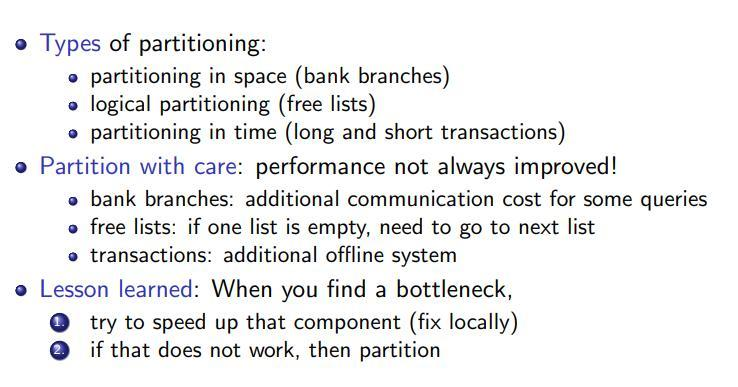
\includegraphics[scale=0.8]{bottleneck.jpg}  
\end{center}
\item start-up costs are high runnig costs are low
Meistens ist die Anstartzeit lange zum bsp beim starten eines Autos, oder Glühbirne die die größte Energie benötigt beim ein und ausschalten.\\
Bei Datenbank Systemen ist das nicht anders.\\
\item [-]Wenn man Daten von der Festplatte liest ist es (ressourcen)teuer die operation zu lesen aber dann können mit highspeed Daten übermittelt werden.\\\
-$>$Häufig genutzte Tabellen sollten der Reihe nach angelegt werden.\\
Gilt auch für RAM(random accesed Memory)wenn man daten sequentiell from RAM scant ist das schneller als wenn man es von verschiedenen Orten herholen muss.
\\
\item[-]Netzwerk Latenz 
Sehr großer Overhead beim senden von Nachrichten.
Kaum zusätzliche Kosten vom senden von großen Nachrichten im Vergleich zu kleinen Nachrichten.\\
--$>$ einige größere Datenpakete zu schicken ist besser als mehrere kleine.\\
Query overhead: bevor eine Anfrage ausgeführt werden kann, wird sie zuerst geparsed,optimiert, und die Datenpfade müssen ausgewählt werden. \\
die Ergebnisse der open genannten Instruktionen können gecached werden.\\
\item[-]Connection Overhead: Beim Verbindungaufbau entstehen hohe Kosten: netzwerk verindung aufbauen, user bestätigen, Verbindungsparameter eroieren.\\
Es ist meistens sinnvoler ein SELECT zu machen und über die Ergebnisse zu iterieren als mehrmals SELECT in einer loop aufzurufen um ans Ergebniss zu kommen\\
--$>$ Das Ziel ist es den benötigten Effect den man braucht mit so wenigen Starts wie möglich zu schaffen.

\item render on the server what is due on the server\\
Relative Datenverarbeitung von Client und Server\\
Wenn der Server überladen ist dann übergibt man Aufgaben dem Client um den Server zu entlasten. Bsp: CPU\\
Da die relevanten Informationen am Server sind ist eine Server Lösung effizienter, wie zb mit einem trigger der nur dann auslöst wenn Veränderungen gemacht werden.\\
Im Grunde ist es wichitg die Arbeit wichtig aufzuspalten und nicht Sachen am Client machst der eig auf dem Server erledigt gehört.\\
\item be prepared for trade -offs \\
Die Geschwindigkeit zu erhöhen ist nicht gratis.
Es kostet neue main memory,speicherplatz, neue CPUs etz.\\
Einen Query zu beschleunigen resultiert vlt darin einen anderen zu verlangsamen.\\
Man muss sich immer Konsequenzen bewusst sein und sich überlegen wieviel man bezahlen will/kann um etwas zu beschleunigen.
\end{itemize}


\item \textbf{Explain write-ahead logging and how the logging mechanism can be tuned.} \\

\item \textbf{Query Tuning/Query Processing} \\
Beim Query Tuning wird eine Anfrage neu geschrieben um schneller zu laufen.
Hat keine schlechten Nebeneffekte!
Beim Query Processing gibt es folgende Schritte:
\item[1)]Parser:\\
dbekommt als Input eine SQL query und liefert eine relationale Algebra expression als Output\\
\item[2)]Optimizer\\
verarbeitet die r a expression zu einem query plan.
\\
Ein query plan wird in 3 schritten erstellt:
-equivalente Umformung : Ergeben das selbe Ergebniss aber die Ausführzeit variiert oft stark.
-Bschriftung der Notation der algebra expression. Eine algebra expression ist kein Query plan : es muss genauer Überlegt werden. zb welchen index man nimmt für joins oder selects, welchen Algo man nutzen will: Hash join oder sort-merge, pipelinig, etz..
-Kosteneinschätzung
Sehr schwer da man nur schätzen kann und es eine große Anzahl an query plans gibt.
Heuristiken anwenden um vielversprechende query plans auszuwählen.\\
\item[3)]Execution engine\\
der query plan wird ausgeführt und liefert das Ergebniss des Querys zum User.\\ \\
\newpage
Query Tunig:\\
Vermeide unnötige Temporäre Tabellen wenn zb auch Index genutzt werden kann.\\
Verwende kein HAVING wenn WHERE verwendet werden kann.\\
Views nur mit Vorsicht nutzen, mit Views werden Queries vereinfacht dargestellt bzw "verpackt", jedoch sind sie nie schneller sondern manchmal sogar langsamer.
\begin{center}
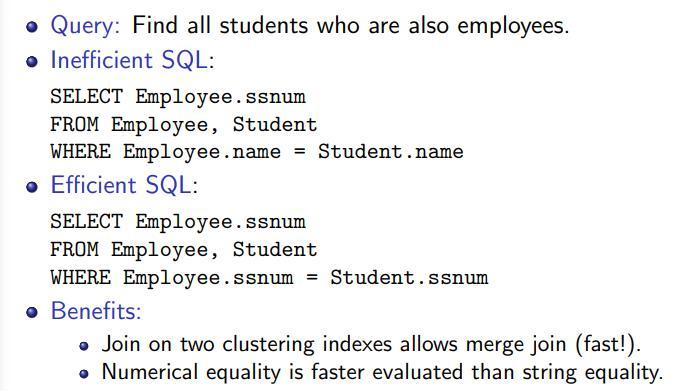
\includegraphics[scale=0.8]{query_tuning.jpg}
\end{center}

Ein Beispiel aus den Folien.
Wenn man zwei einen Join auf zwei geclusterte Indexe ausführt kann man einen merge join machen welcher (sehr!)schnell ist.\\
Weiteres ist es schneller numerisch nach der \textit{ssnum} zu suchen als nach einem String (name)\\
Sometimes use UNION statt OR.


\item \textbf{How to avoid DISTINCT. Give an example of a nested query and rewrite it. Explain different nested query
types.
} \\ \\
\textit{DISTINCT} entfernt Duplikate aus den Ergebnissen des Querys.\\
\textit{priviliged} table: Die Attribute die durch SELECT zurückgegeben werden besitzen einen Schlüssel (contain a key).
\begin{verbatim}
SELECT ssnum
FROM Employee, Techdept
WHERE Employee.dept = Techdept.dept
\end{verbatim}
Employee ist eine priviligierte Tabelle, select stellt ssnum dar welches ein key von Employee ist.\\
\textit{Reachability} Man hat 2 Tabellen R und S .
R reaches S wenn R und S gleichermaßern verbunden sind und das join Attribut in R ein key von R ist.\\
Ein Tupel von S ist mit mindesten einem Tupel von R verbunden.\\
Reachability ist transitive.\\
Diese Anfrage gibt vlt Duplikate zurück:
\begin{verbatim}
SELECT ssnum
FROM Employee, Techdept
WHERE Employee.manager = Techdept.manager
\end{verbatim}
Weil manager kein Schlüssel von Techdept ist.\\
Daher erreicht Techdept nicht den privilged Table von Employee.\\------------------------------------------------------------------------------------------ \\
Diese Query gibt \underline{keine} Duplikate zurück:
\begin{verbatim}
SELECT ssnum, Techdept.dept
FROM Employee, Techdept
WHERE Employee.manager = Techdept.manager
\end{verbatim}
Sowohl Techdept als auch Employee sind priviligierte Tabellen.\\ vermeiden indem man schaut ob es sich um einen priviliged table handelt weil dann hat man einen key der einzigartig ist und mit dem man in der Query dann garantiert keine Duplikate bekommt, weiters muss man auf die Reachabillity achten also es kann sein das vlt 2 Tables keine gemeinsamkeiten haben können trotzdem dank transitivität und geschickten querys alle Tabellen erreicht werden.\\ \\
Nested Querys:\\
Eine nested Query oder sub-query ist Select Abfrage innerhalb einer WHERE Abfrage.\\
Eine Subquery liefert ein Ergebniss um dies dann an die Haupt-Query weiterzuverwenden.
\textbf{\textit{Correlated} subqueries}
Ist eine nested query welche Werte von der äußeren Query hernimmt um etwas zu berechnen.
Daher dies einmal für jede Zeile berechnet werden muss kann es sehr langsam sein.
\textbf{\textit{Un-correlated} subqueries} 
Ist eine nested Query welche keinen Bezug zur äußeren Query hat und ihre Abfrage ganz allein  ausführt.\\ \\
Rewritting a nested Query:\\
Step 1) Man kreiert eine temporäre Tabelle:\\-GROUP BY von zusammenhängenden attributen von der nested Query.(diese müssen gleich sein)\\
-Verwende nicht zusammenhängende Voraussetzungen von der sub-query um die temporäre Tabelle zu kreieren.\\
in diesem Fall : Employee.dept = Techdept.dept ist die qualification.\\
Step 2) Man joint die temporären Tabelle mit der äuseren Abfrage welches die condition ersetzt : Techdept.dept wird zu Temp.dept\\
Das \begin{verbatim}
SELECT ssnum
FROM Employee e1, Techdept
WHERE salary = (SELECT AVG(e2.salary)
FROM Employee e2, Techdept
WHERE e2.dept = e1.dept
AND e2.dept = Techdept.dept)
\end{verbatim}
wird zu
\begin{verbatim}
SELECT ssnum
FROM Employee e1, Temp
WHERE salary = avsalary
AND e1.dept = Temp.dept;
\end{verbatim}

\item \textbf{Explain the different types of subqueries and how they can be tuned. Rewrite the following subqueries:} \\TODO\\
\item \textbf{Explain the different Query Types.}\\Für jeden query Typen braucht es bestimmte indexe.\\
Wir unterscheiden zwischen folgenden Query Typen: \item[-]\textit{Point query: }returnt höchstens einen Eintrag.
\begin{verbatim}
SELECT name
FROM Employee
WHERE ID = 8478
\end{verbatim}
\item[-]\textit{Multipoint query: }returns mehrere Einträge abhängig von der equality Kondition.
\item[-]\textit{Range query: }auf X gibt Einträge mit Werten im Interval von X zurück.
\item[-]\textit{match query: }Man gibt eine bestimmte geordnete sequence von Attributen vor und filtert sich so den gewünschten Wert raus:
z.b : lastname ='Gates' AND firstname= like 'Ge\%'
\item[-]\textit{Extremal query: }gibt Einträge von max oder min Werten von ausgewählten Attributen zurück.
\item[-]\textit{Ordering Query: }ordnet die Einträge nach bestimmten Attribut Werten.\\
z.b SELECT * FROM Employee ORDER BY salary
\item[-]\textit{Grouping query: }Zerlegt die Einträge in Gruppen(meistens ist jede Partition mit einer bestimmten function versehen z.b AVG()\\SELECT dept, AVG(salary)
FROM Employee
GROUP BY dept
\item[-]\textit{Join querys: }Es werden zwei oder mehr Tabellen verknüpft\\
\item[-]\textit{prefix querys: }Geht durch den Baum und findet prefix und folgt den pointern zwischen den Index Knoten.
\\ \\
\newpage
Was ist ein INDEX ?\\
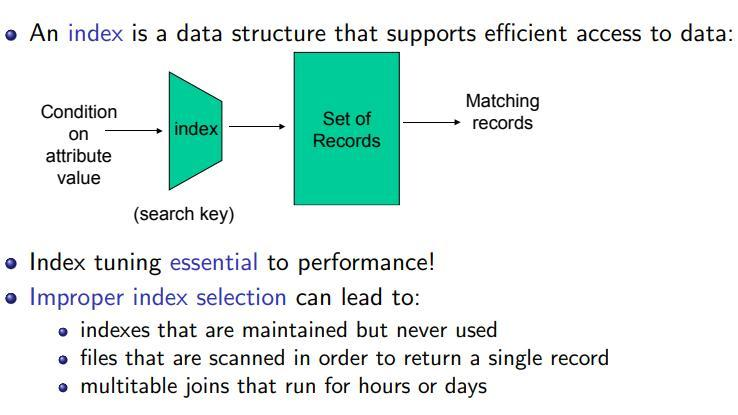
\includegraphics[scale=0.8]{what_is_an_Index.jpg}\\
Der Key oder Schlüssel von einem Index ist zu unterscheiden:\\
-search key: ist ein einzelnes oder eine Folge von Attributen die dazu da sind Werte in Tabellen auszulesen.\\
-sequential key: Der Wert ist gleichbleibend, z.b counte, timestamp.\\
non-sequential key: Der Wert ist hat keine Ordnungsnummer wie z.b ssnum , last name.\\ \\
Der Index key ist nicht gleich unique also er ist nicht unbedingt ein key attribute wie in der Relaationalen Theorie.\\\\
Index Characteristics: Ein Index kann oft als Tree gesehen werden (Hash, B$^+$tree)\\
Dabei sind manche Knoten im Hauptspeicher und andere weiter unten liegende eher nicht.\\
Fanout bezeichnet die Anzahl an Kinder die ein Knoten haben kann eine große fanout bedeuted wenige Levels.\\
Overflow Strategies: in einen vollen index einen knoten n einfügen \\
ein neuer Knoten n' muss zur disk zugewiesen werden.\\
B$^+$-tree: teilt n in n und n' auf beide mit der selben Distanz zur Wurzel.\\
hash index: n speichert pointer zu einem neuen Knoten n'(overflow chaining)
\item \textbf{What are dense, sparse, clustering and non-clustering indexes? Discuss their advantages and disadvantages and
when to use them.} \\
-Sparse index: Zeiger zu Festplattenspeicher mit höchstens einem Pointer pro Festplattenspeicher seite., meistens gibt es weit weniger pointers als Einträge\\ \\
-Dense index:Es existieren Zeiger zu individuellen Einträgen mit je einem Schlüssel pro Eintrag.
Dense hat meistens mehr Schlüssel als Sparse weil es für jeden Eintrag einen gibt. Eine Optimierungsmöglichkeit ist es sich wiederholende Schlüssel nur einmal zu speichern mit Zeiger versehen.\\
Die Anzahl an Pointers im  dense index ist gleich der Anzahl an pointers im sparse index * die Anzahl an Einträgen pro Seite.\\
Der Vorteil an \textit{sparse} ist das es weniger pointer gibt und weniger pointer resultieren in weniger levels und verwenden dadurch weniger Speicher.\\
Der Vorteil \textit{dense }index ist es das dieser abdeckend eingesetzt werden kann und sogennante "cover" quereys unterstützt, dass sind Lese-Anfragen (read querys) innerhalb der Datenstruktur, die aber nicht auf die Dateneinträge zugreifen sondern diese nur lesen.$\rightarrow$ fast!\\ \\
Innerhalb einer Tabelle kann es deswegen logischerweise nur einen sparse index geben aber mehrere dense Indexe.\\ \\
\underline {clustering und non-clustering Index:}\\
Clustering bedeutet geordnet, das heißt die Einträge sind nach einem Attribut X gruppiert.\\
Beim B$^+$ Tree sind die Einträge nach Attribut X sortiert.\\
Es gibt nur eine geclusterten index pro Tabelle  der dense oder sparse ist.\\
\underline{non-clustering:}\\ Keine Beschränkung von Tabellenorganisation.\\
Es gibt mehr als einen Index pro Tabelle der immer dense ist.\\ \\
Clustering Indexes können sparse sein und sind gut für multi-point querys um zb den letzen namen einer liste zu bekommen oder wenn der geclusterte index als B$^+$-tree implementiert ist nach Nachnamen mit dem prefix "Jo" zu filtern.
Die Ergebnisse sind in darauffolgenden Seiten was zu Overflow pages führen kann wenn die Disk-page voll ist weil dann die überschüssigen Einträge zu den überlaufenden pages sollen.\\
Where to use:
\begin{verbatim}
SELECT Employee.ssnum, Student.course
FROM Employee, Student
WHERE Employee.firstname = Student.firstname
\end{verbatim}
Index auf Employee.firstname mit einer index nested loop join, wo man für jeden Student die Employees mit dem selben Namen checkt.
Schneller geht es mit einem Index auf beide $.$firstname Attribute mithilfe von einem Merge Join.\\
Wir lesen beide Tabellen in sortierter Reihenfolge und mergen diese ($B^+$-tree), dadurch muss man jede Tabelle nur genau einmal lesen.\\ \\
Der Clustering Index ist um einiges schneller als der non-cluster index.
Der non-clustering Index ist jedoch immer sinnvoll für zb point queries wo nur ein bestimmtes resulatat gesucht wird insbesonders in Verbindung mit Index covers Query.\\
Der vorhin genannte Overflow der passieren kann weil ein clustering index immer die Einträge auf einer nachfolgenden Seite speichert kann zb gelöst werden, indem man $A->B->C$ zu $A->B'->B''->C$ umwandelt, also die B Ergebnisse aufteilt.

\item \textbf{Discuss $B^+$-tree and hash-index. Which queries are supported?}\\
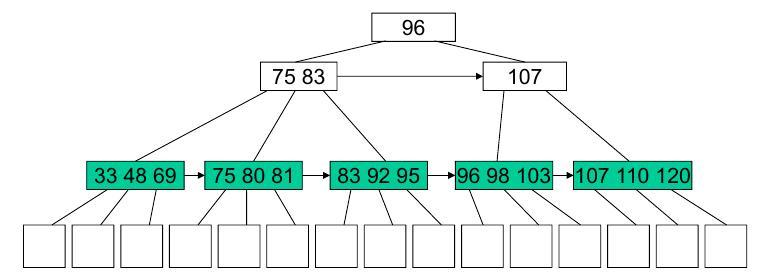
\includegraphics[scale=0.7]{BplusTree.jpg}
Der \textbf{B$^+$-Tree} ist ein balazerter Baum mit Schlüssel-pointer Paaren, welche sortiert sind.\\
Die Knoten müssen mindestens halb voll sein.
Der Zugriff auf die Datensätze erfolgt von der Wurzel zum Blatt.\\
Es ist wichtig eine möglichst kurze Key-Length zu haben um ein möglichst großes fanout zu bekommen.\\
Die Anzahl an Levels berechnet man sich mit dem fanout = $\frac{nodesize}{keypointer-size}$ (abrunden)welche man dann einsetzt:\\
Anzahl an Levels = $\log_{fanout*Page Ausnutzung}$(Blatt Schlüssel-pointer Paare)\\
\\Mithilfe von Key-Kompression(kostet CPU time) kann man lange Keys kürzen.
Sehr hilfreich bei String Keys mit zb. der Prefix Compression.\\Cagliari, Capri $\rightarrow$ Cag, Cap.\\ \\
\textbf{Hash-Index} Eine \underline{Hash Funktion} mappt Schlüssel zu Integer Werten von $[0...n]$ (hash values)\\
Die Schlüssel sind über den ganzen Bereich verteilt und ähnliche Schlüssel haben oft trotzdem sehr unterschiedliche hash-values.\\
Die Hash Function agiert als "root node" vom Index Tree. Das Hash Value ist eine Bucket Number die auf buckets zugreift(haben fixe Größe).\\ Wenn ein Bucket voll ist wird ein Overflow Bucket erstellt auf den zugegriffen wird indem man dem Pointer folgt der im vollen Bucket gespeichert ist.\\ \\
\underline{Which Queries are supported?}\\
$B^+$-tree unterstüzt so ziemlich jeden query type: point, multi-point,range, prefix, extremal,ordering, grouping.
Hash-Index unterstützt nur point (single disk access), multi point(single disk access to first record) und grouping(grouped records have same hash value)\\
Hash-Index ist ungeeignet  für range, prefix, extremal und ordering.\\
Weil ähnliche Key Werte unterschiedlich Hash Werte haben und daher auf verschiedenen Seiten liegen.\\
Bei einer Point query eignet sich ein Hash Index am besten da der nicht auf die Disk zugegriffen werden muss und der key einzigartig ist, bucket overflow is unwahrscheinlicher.\\
Bei einer Multipoint query eignet sich am besten ein $B^+$Tree weil die Einträge auf aufeinander folgenden Seiten sind.(sowie range query). \\Bei Hash problematisch weil dann alle relevanten Einträge in einem Bucket sind. $\rightarrow$ overflow chain.\\ \\
Composite Indexes sind Indexe auf mehr als ein Attribute also z.b auf lastname,firstname.
Ist oft effizienter als zwie single-attribute indexe, vorallem effizeint für Prefix querys.
Im $B^+$Tree kann es zu sehr vielen Layern kommen aufgrund der großen Keysize.

\item \textbf{Explain the different join strategies (+ Rechenbeispiel, ob sich ein HashJoin am Beispiel lohnt; Beispiel war
1:1 aus den Folien)}\\

geg: Relation R(outer) und S(inner):\\
R:$ n_{r}$ = 5000 records, $b_{r}$ = 100 disk blocks, 0.4MB\\
S: $n_{s}$ = 10000 records, $b_{s}$ = 400 disk blocks, 1.6MB
\begin{itemize}
\item Naive Nested Loop join:\\
Nimmt jeden Eintrag von R und durchsucht alle Einträge von S nach Übereinstimmungen.
\item Block Nested Loop Join:\\
Vergleicht alle Reihen von jedem Block von R mit allen Einträgen in S.
S wird für jeden Eintrag in S einmal gescannt.
\item Indexed Nested loop join: \\Durchsucht jede  Reihe von R nach Übereinstimmungen in S mithilfe eines Indexes.\\
Es ist effizient wenn es ein index cover join ist, oder wenn R weniger Einträge als S hat pro Seite.
\item Merge Join(zwei geclusterte indexe):\\
scant R und S in sortierter Reihenfolge und fügt diese zusammen(merge), R und S werden je nur einmal gelesen.
\item Hash Join(equality, no index):
Man hashed beide Tabellen in Buckets mit der selben Hash Funktion.\\
joint die Paare von zusammengehörigen buckets in der main memory.

\end{itemize}
\item \textbf{Explain write-ahead logging and how the logging mechanism can be tuned. (Musterfrage in Folien)} \\
Lösung für das Recovering.
\underline{WAL commit:} 
Bei einem commit werden hier nur die after images persistent im log gespeichert.\\
Die anderen data diles werden irgwann später geupdated.\\
\underline{WAL abort:}
Es gibt zwei Varianten:
\item[1] das before image wird explizit gespeichert. 
\item[2] verwenden das auf der datenbank gespeicherte before image.\\
Es muss aber sichergestellt werden das diese before Bilder sicher nicht überschreiben werden.\\generell werden dirty pages zurück auf die disk geschreiben wenn der Puffer im Hauptspeicher voll ist. $\rightarrow$ deswegen wird meistens Variante 1 benutzt.\\
Tuning of logging system:\\
\item[1] Log on seperate Disk:
Update Transaktionen: werden immer in den Log geschrieben also auf die Disk.\\
Wenn log und data files auf der selben Disk liegen kommt es zu Disk seeds.\\
Seperate disk for log: sequentielles schreiben und lesen ist um ein vielfaches schneller.
Weiteres kann man über den Puffer im Hauptspeicher aussteigen um Partial writes zu vermeiden.
\item[2]Group Commit: Man schreibt eine vollständige Seite vom Log Buffer auf die Festplatte in dem unter anderen das Before Image enthalten ist.\\
Die Seiten sind jedoch oft ned voll, deswegen bündelt man diesen eine Schreibvorgang um den Durchsatz des Systems zu erhöhen.\\
Der Nachteil ist das einzelne Transaktionen auf ihre commits warten müssen, und unter anderen ihre Datensperre behalten.\\ \\
WAL Buffer und Group Commit:
Man kann die Write-ahead loggin Puffergröße und deren flush intervall verändern. Je größer der Puffer desto mehr Änderungen passen hinein\\
Intervall erhöhen wann eine Pufferseite auf die Festplatte geschrieben wird.
Es kann einzeln eingestellt werden wie lang eine Transaktion maximal warten soll bis die group voll ist und wie groß die group sein soll.
\item[3]WAL Tuning: synchronous:commit: ist on\\
Alle Durability Anforderungen vollständig.
Dies wird erreicht indem das Commit an die Transactions erst gesendet wird wenn fsync alle Daten erfolgreich in den persistenten Speicher geschrieben hat.\\
Die Idee ist es nicht zu warten bis das passiert ist sondern das commit schon während des Schreibvorgangs an den Client der die Transaktion gestartet hat zu senden.(Dies kann für jede Transaktion einzeln eingestellt werden)\\
Worst-case:keine inkonsitente Db, aber es könnten teile der Transaktionen in data files enthalten sein.\\Das Problem ist das der Client immer noch denkt das seine Transaktionen in der Db dauerhaft gespeichert sind.
Die risk period ist die Zeit zwischen dem gesendeten commit und dem tatsächlichen commit.\\
Die zeit lässt sich berechnen mit 3* wal_write_delay.\\
Ohne fsync könnte die Db in einem inkosisten Zustand endet.\\
\item[4]Tuinig Data Writes: \\
Beim commit müssen alle zu commiteten Seiten aus dem Puffer und den logs in die Data files geschriebn werden.\\
Nicht unmittelbar weil der Schreib Lese Kopf erst an die richtige Stelle der Festplatte bringen.\\
Sinnvoll ist es die Schreibvorgänge zu bündeln so das möglichst viele Seiten geschrieben werden. Weiteres kann man eine Seite genau dann schreibn falls sich der Schreibkopf genau dann an der richtigen Stelle befindet.\\
Desto weniger checkpoints desto mehr dirty pages sind im puffer.\\
Kommt es zu zuvielen checkpoints kann man sich mit checkpoint_warnings(30s) warnen lassen und wenn nötig sollte man dann die max_wal_size zu erhöhen.\\
jedoch bei kostet der Wiederstart ohne checkpoints nach einem Fehler länger als mit checkpoints diesen Tradoff ist zu Tunen.

\item \textbf{Erklaeren der unterschiedlichen Disk-Allocation Methoden. RAIDs erklaeren und welches RAID fuer welche
File-Typen empfohlen wird. } \\
\item \textbf{} \\
\item \textbf{} \\
\item \textbf{} \\
What is transaction chopping and how does it work? Show the algorithm on the following transactions: T1:
R(a),R(b),W(b),R(e), T2:R(b), ... (Musterfrage in Folien)
Explain the different types of subqueries and how they can be tuned. Rewrite the following subqueries: ...
(SQL-Code ähnlich den Folien)

Erklaeren der unterschiedlichen Disk-Allocation Methoden. RAIDs erklaeren und welches RAID fuer welche
File-Typen empfohlen wird. 
Diskutiere die verschiedenen Join Strategien (die genaue Funktionsweise und die Anzahl der Lese- und
Schreibzugriffe). Lohnt sich ein non-clustered Index bei folgendem Beispiel: In der Tabelle Employee sind 200
Angestellte eingetragen, die jeweils einem von 50 Departments zugeordnet sind. Wobei ein Block 4KB groß ist
und ein Employee Eintrag 200B benötigt. In der Tabelle TechDepts sind 10 dieser Departments eingetragen.
Diskutiere die verschiedenen Isolation Guarantees (SQL Standard) und erkläre wie Snapshot Isolation in
Oracle umgesetzt wird.




\end{enumerate}

\end{document}
